\documentclass[conference]{IEEEtran}
%\documentclass{article}
\usepackage{cite}
\usepackage{amsmath,amssymb,amsfonts}
\usepackage{algorithmic}
\usepackage{graphicx}
\usepackage{textcomp}
\usepackage{xcolor}
\usepackage{tabularx}
\usepackage{tikz}
\usepackage{pdfpages}
\usepackage{url}
\usepackage{makecell}
\usepackage{caption}

\newcommand{\CoBBl}{\textsc{CoBBl}}
\renewcommand{\P}{\mathcal{P}}
\newcommand{\V}{\mathcal{V}}
\newcommand{\C}{\mathcal{C}}
\newcommand{\red}[1]{{\color{red}#1\color{black}}}
\newcommand{\code}[1]{\texttt{#1}}
\newcommand{\comment}[1]{\color{teal}\texttt{#1}\color{black}}
\renewcommand{\sp}{\mathsf{\%SP}}
\newcommand{\bp}{\mathsf{\%BP}}
\newcommand{\bn}{\mathsf{\%BN}}
\newcommand{\addr}{\mathsf{addr}}
\newcommand{\val}{\mathsf{val}}
\newcommand{\ls}{\mathsf{ls}}
\newcommand{\ts}{\mathsf{ts}}

\def\BibTeX{{\rm B\kern-.05em{\sc i\kern-.025em b}\kern-.08em
    T\kern-.1667em\lower.7ex\hbox{E}\kern-.125emX}}

\title{\CoBBl: Dynamic SNARK Constraints using Basic Blocks}
\author{Kunming Jiang, Riad Wahby, Fraser Brown}
\date{October 1, 2024}

\begin{document}

\maketitle

%\begin{abstract}
SNARK (succinct non-interactive argument of knowledge) is a cryptographical protocol widely adopted in cloud computing and blockchain that allows verification of a computation in sublinear time. Existing SNARK systems can be largely divided into two approaches. The compiler approach converts the program into a set of static constraints and generate a proof based on the satisfiability of the constraints, while the virtual machine directly asserts correctness on the sequence of assembly instructions executed by the computation. 

This paper introduces $\CoBBl$, a new SNARK protocol that combines the two existing approaches. Through introducing and modifying the concept of basic blocks, $\CoBBl$ achieves all optimizations present in existing SNARK compilers, while allowing the proof to contain dynamic constraints according to the execution path.
\end{abstract}

\section{Introduction}

A SNARK (succinct non-interactive argument of knowledge) is a cryptographical protocol that allows an untrusted prover $\P$ to convince a verifier $\V$ that it knows a witness $z$ that satisfies certain properties. Trivially, $\P$ can convince $\V$ by sending the entirety of $z$. Through the usage of SNARK, however, $\P$ can produce a proof with shorter length than $z$, and $\V$ can verify the proof faster than reading the entirety of $z$. One popular usage of SNARK is to verify the correct execution of computer programs, which allows users to outsource computations to untrusted parties in cloud computing and blockchain settings.

Early works \cite{setty12ginger, wahby14buffet, kosba18xjsnark, ozdemir20circ} of SNARK primarily focus on program translation. In these \emph{direct-translator} approaches, a program is first converted, in a trusted preprocessing phase, to a set of arithmetic constraints that are satisfiable if and only if the prover $\P$ correctly executes the program. \red{[XXX: Need to emphasize the importance of constraint size.]} Next, $\P$ convinces the verifier $\V$ that it holds an assignment that can satisfy the constraints. Since constraint satisfiability is equivalent to correct program execution, $\V$ accepts the output of the program provided by $\P$. Direct-translators have the advantage of utilizing the semantics and structure of a program to produce the constraints most \emph{tailored} to a specific, which can often lead to massive cost reduction. However, the downside is that the constraints produced need to be \emph{fixed at compile time}, and thus have to take into account all execution paths of the program. In practice, proofs generated by direct-translators need to pay for both branches of a conditional statement, and infer and unroll every loop up to a statically-determined upper bound on number of iterations. These proofs often contain \emph{wastes} -- work that do not correspond to any executed instructions --  increasing compiler, prover, and verifier time.

Later works \cite{zhang18vram, arun23jolt} explore a new type of SNARK focusing on CPU emulation. Commonly referred to as the \emph{virtual machine (VM)} approach, these systems represent any program execution trace with an instruction set architecture (ISA) like TinyRAM or RISC-V assembly, and express correct program execution through correct execution of individual instructions. They achieve so by pre-generating constraints used to verify each instruction in the ISA, and when later given $\P$'s execution trace, map each instruction in the trace to the corresponding constraints. As such a proof contains only instructions executed by $\P$, it avoids wasted work incurred by direct translators. However, since all constraints are pre-generated, \red{[XXX: How to express the idea that constraints NEED to be fixed at compile time?]}, SNARK systems employing the VM approach cannot apply program-specific tailoring, conceding a major advantage to their direct-translator counterparts. Furthermore, these systems often require additional wirings in-between the instructions to ensure consistent program states throughout the execution, introducing additional overheads per instruction.

The advantages and drawbacks of the aforementioned two approaches naturally raise a question: \emph{can a SNARK system emit constraints tailored to each specific program like a direct-translator, while paying only for executed instructions like a VM?} We show an affirmative answer by introducing \CoBBl, a middle path between the direct-translator and VM approaches that absorbs the advantage of both worlds. \CoBBl~makes the following innovations and contributions:
\begin{enumerate}
    \item A SNARK compiler that divides a program into segments and converts each part into constraints.
    \item An optimization toolkit that infers the optimal segmentation of a program, and the optimal constraint representation of each segment.
    \item A proof protocol that specializes in program segment verification, based on Spartan \cite{setty19spartan}.
\end{enumerate}

%\section{Preliminaries}
To present the general framework in which \CoBBl~operates, we begin with a few building blocks and general definitions.

\paragraph{SNARK} SNARK (succinct non-interactive argument of knowledge) is a cryptographical protocol in between two parties: a prover $\P$ and a verifier $\V$. The input of the protocol is a set of constraints $\C$, to which $\P$ purportedly holds a satisfying assignment $z$. The protocol itself involves $\P$ utilizing a randomized algorithm to generate a proof of knowledge, which $\V$ can apply the same randomness to verify in time sublinear to the size of $\C$.

\paragraph{Verifiable Computation (VC)} In a VC setting, a verifier $\V$ outsources a computation $f(x)$ to an untrusted prover $\P$. $\P$ returns the purported output $y\xleftarrow{?} f(x)$ together with a SNARK proof $\pi$ on the correctness of $y$. $\V$ checks the proof and either accepts or rejects $y$. In particular, the above protocol needs to satisfy three requirements:
\begin{itemize}
    \item \textbf{Completeness}: If $y=f(x)$, then $\V$ always accepts $y$.
    \item \textbf{Soundness}: If $y\neq f(x)$, then $\V$ rejects $y$ except for negligible probability.
    \item \textbf{Succinctness}: The size of $\pi$ and $\V$'s work should be sublinear to the execution of $f(x)$.
\end{itemize}

\paragraph{Frontend and Backend} SNARK systems are usually divided into two phases: the frontend that generates constraints, and a backend that generates proofs from the constraints. The frontend of compiler-style and VM-style SNARKs are substantially different. However, since these frontends ultimately all emits arithmetic constraints, different SNARK systems can share the same backend.

\paragraph{Data-Parallelism} Many SNARK backend systems support data-parallelism, which verifies multiple SNARK proofs at once, with time sublinear to sequential verification. Data-parallelism usually requires the proofs to share some common properties like number of constraints and witnesses.

\paragraph{Basic Blocks (BB)} A basic block is a sequence of code in a program that contains no control flow in-between. In other words, the execution of the first instruction in a BB implies the execution of every instruction in that BB. BBs are frequently used by compilers as the basis for analyses and optimizations, and a program can be expressed as a control flow graph of its BBs.

%\section{The Case for a New SNARK Framework}
The goal of \CoBBl~is to explore a middle path between compiler-style and VM-style SNARKs. To achieve so, it takes inspirations from two existing systems from the two approaches: CirC and vRAM. To illustrate the design of \CoBBl, we first provide brief descriptions of our two predecessors.

\subsection{CirC}
CirC is a compiler infrastructure that provides a link between high-level programming languages and arithmetic or logical circuits like R1CS or SMT. To achieve so, CirC translates a program of a high-level language into a state-free, non-uniform intermediate representation (IR) called CirC-IR. In the context of verifiable computation, these IRs are then lowered into R1CS in a standardized process in-line with those introduced by earlier works \cite{setty12ginger, wahby14buffet, kosba18xjsnark}. Additional optimizations like linear-reductions are deployed to minimize the size of the R1CS constraints.

We build the frontend of \CoBBl~largely based on CirC. In particular, \CoBBl~utilizes CirC's translation to and from CirC-IR for its own constraint generation. However, unlike CirC, which translates a flattened version of the entire program into IR, \CoBBl~invokes additional preprocessing that divides the program into segments, before converting individual segments into IR and R1CS.

\subsection{vRAM}
vRAM is a VC system with a circuit-independent preprocessing stage. This means that vRAM does not require any compile-time setup on the program to be verified. Instead, vRAM only requires a one-time setup that generates constraints for every TinyRAM instruction type. For proofs, $\P$ expresses any execution of any program as an \emph{execution trace}: a sequence of program states $[S_0\dots S_T]$, where the first state $S_0$ is the program input, and all subsequent states $S_{i+1}$ are generated by applying a TinyRAM instruction $I_i$ to the previous program state $S_i$. To verify the correctness of the trace, $\V$ checks the following:
\begin{itemize}
    \item All instructions are fetched correctly.
    \item All instructions are executed correctly.
    \item All memory accesses are coherent.
\end{itemize}

In order to achieve sublinear verification time, vRAM uses data-parallelism to generate a batched proof on all instructions. In concrete terms, it invokes the following procedures:
\begin{enumerate}
    \item For every state $S_i$ and instruction $I_i$, $\P$ appends the output of the instruction, $O_i$, to the end of $S_i$. The pair $(S_i, O_i)$ form the witnesses for verifying the correct execution of $I_i$.
    \item For every consecutive pair of program states $(S_i, O_i, S_{i+1})$, $\P$ proves that the corresponding register in $S_{i+1}$ is updated to $O_i$ and everything else stays the same.
    \item For instruction correctness, to minimize proof size, $\P$ first permutes the list of $(S_i, O_i)$ by the type of $I_i$, then verifies that $O_i$ is the correct output of applying $I_i$ on $S_i$. The permutation allows the proof to only include one copy of constraints for each type of instruction executed. We cover this process in more details in section \ref{sec:block_correctness}
    \item Finally, constraints of memory operations extract out all memory accesses. Through a separate permutation, $\P$ proves memory coherency in an approach first introduced by Buffet \cite{wahby14buffet}.
\end{enumerate}

The final proof of vRAM is consisted of four components:
\begin{enumerate}
    \item Pairwise program state consistency check.
    \item Permutation of $(S_i, O_i)$ from execution-order to instruction-order.
    \item Batched instruction correctness check.
    \item Memory coherence check.
\end{enumerate}

We apply this high-level idea of 4-component proof to the proving structure behind \CoBBl, with major changes in each component to match the output of the \CoBBl~frontend.

\subsection{Motivating for a new SNARK system}
While CirC and vRAM are highly efficient in their own regards, they also introduce different overheads in the process. The CirC compiler, as described briefly in the introduction, generates a flattened, static IR for the program. The constraints lowered from such IR need to account for all execution paths, which leads to two problems:
\begin{enumerate}
    \item The constraints need to express all branches of a conditional, even though only one would be taken in any execution. This creates "wastes" in the proof, \emph{i.e.} constraints that do not correspond to an executed instruction.
    \item All loops within the program needs to be flattened and unrolled. Such a process results in constraint size linear to the execution trace, as opposed to size of the code, inflating the work of the compiler and preprocessor. Further more, loops without an explicit upper bound on number of iterations require hints from the programmer for unrolling; if supplied incorrectly, can compromise proof completeness and soundness. 
\end{enumerate}

vRAM solves the above problems by verifying the execution trace and eliminating program-specific preprocessing. In order to do so, however, vRAM introduces program state consistency check. Every instruction $I_i$ in the execution trace translates to one additional $(S_i, O_i)$ entry in the program state permutation and one additional consistency check between $S_i$ and $S_{i+1}$. Both overheads require linear scan on the program state. For cheap instructions like addition and multiplication, verifying permutation and consistency can be more costly than the instruction itself.

%\red{Detailed runtime comparison?}

%\section{Interpolating CirC and vRAM} \label{sec:framework}

We set up \CoBBl~by first generalizing the achievements of CirC and vRAM. CirC's optimizations are enabled by its static analysis. To retain these optimizations, \CoBBl~requires a frontend compiler. vRAM avoids constraint waste thanks to its design that permits control flow in-between its constraints -- a feature that \CoBBl~needs to incorporate.

The presence of the compiler necessitates program-specific preprocessing, while inter-constraint control flow implies that the program needs to be segmented in a way that reflects its control flow graph. It turns out there is a natural candidate for the above two requirements: compilers like LLVM \cite{lattner02llvm} perform optimizations by first dividing the code into \emph{basic blocks (BB)}. We note that expressing an execution trace in terms of BBs have the following desirable properties:
\begin{enumerate}
    \item Each BB contains no control flow in between its instructions. Thus, if the basic block were to be executed, no constraint representing it would be wasted.
    \item Typical BBs often span multiple instructions, resulting in reduced number of program states in the trace comparing to the VM approach.
    \item There exist extensive researches in the compiler community \cite{sui16svf, lee18recon} on optimizations within and between basic blocks, which can be easily incorporated into the \CoBBl~compiler.
\end{enumerate}

Despite the stated advantages, basic blocks also come with imperfections. For one, size of BBs of a program can be vastly different. Verifying the instructions of the smallest blocks might still not justify the cost of permutation and program state consistency. Furthermore, data-parallelism in the backend requires all witnesses to be of the same size, leading to extensive padding.

% Size of BBs of a program can be of vastly variable size, which translates to huge differences in number of constraints and intermediate variables. An ideal data-parallel proof, however, expects the size of constraints and witnesses to be similar across all instances.

To improve upon BBs, we observe that the trade-off between constraint wastes and program-state check is in fact a continuous spectrum, with CirC and vRAM sitting on either ends of it. While the basic block approach presents itself as a middle path between the two, it is far from being the only alternative. Since conditionals can be translated into constraints, there is no reason why program segments of a SNARK proof need to strictly follow the rules of BBs. Starting from basic blocks, \CoBBl~performs block merging and register spilling to maximize average proof efficiency. We describe details of these processes in section \ref{sec:frontend}. The optimized block are then converted into constraints, which are subsequently fed into a custom-made data-parallel version of the Spartan protocol \cite{setty19spartan}.

%\begin{itemize}
%    \item By merging or unrolling \emph{short} basic blocks, \CoBBl~reduces the number of program states at the expense of an uptick in number of wasted constraints. However, maximum constraint size remains untouched.
%    \item By spilling variables / registers in between blocks, \CoBBl~trades shortened program state width with increased memory accesses.
%\end{itemize}

%\section{Converting a Program into Constraints} \label{sec:frontend}

As described in section \ref{sec:framework}, the \CoBBl~frontend converts a program into a set of constraints, each corresponding to a segment modified from one or more basic blocks of the program. The entire frontend can be viewed as a three-step process:
\begin{enumerate}
    \item Convert a program into a control flow graph of BBs and perform basic compiler analyses including liveness, alias, and constant propagation. \label{step:convert}
    \item Perform proof-specific optimizations including block merging and register spilling to generate the final set of program segments. \label{step:optimize}
    \item Lower the segments down to a set of IR, then to a set of R1CS constraints. \label{step:lower}
\end{enumerate}

\subsection{Expressing a program using basic blocks}
\CoBBl~converts a program into basic blocks through a linear scan of its instructions. For every conditional or iteration statement, \CoBBl~allocates a new block to reflect an edge on the control flow graph. However, unlike LLVM where variables are assigned new versions for each overwrite, \CoBBl~labels variables by the scope they are defined in. These scope information are later used by register spilling. In addition to the instructions, each basic block also includes a terminator, containing labels of successor blocks and the conditions to reach them.

\subsection{Optimizing blocks for backend}
As discussed in section \ref{sec:framework}, basic blocks still leave rooms for improvement. Below, we identify potential inefficiencies and present \CoBBl's solution for further optimization.

% We introduce further optimizations to minimize the following metrics:
%\begin{enumerate}
%    \item Maximum constraint size of any program segment.
%    \item Average number of wasted constraints.
%    \item Average number of program states, \emph{i.e.} average number of executed segments.
%    \item Program state width, \emph{i.e.} number of variables / registers inside each program state.
%    \item Number of memory accesses.
% \end{enumerate}

% By estimating the changes to the above metrics, \CoBBl~selectively applies optimizations derived from static analyses. Below we present a subset of optimizations performed by \CoBBl.

\paragraph{Block merging} For short basic blocks, the small verification cost for its instructions does not justify the cost to express and check the program state. One simple solution is to merge short BBs together. Block merges reduce the average number of program states at the cost of reintroducing "wastes" back to the proof. To perform block merges, \CoBBl~first establishes a \emph{block size threshold} based on maximum BB size. Block size threshold helps limit the waste introduced by merges. Next, for every short block, \CoBBl~scans for merge candidates. If the merged block is still within the size threshold, \CoBBl~performs the block merge.

\paragraph{Register spilling} \CoBBl~minimizes the number of variables within each program state by excluding out-of-scope variables from the program states. This is achieved through a \emph{scope stack}, where \CoBBl~selectively pushes out-of-scope variables onto it, and pops them out upon scope changes. In more details, for any variable defined in multiple scopes, \CoBBl~initially expresses its value in every scope as separate registers in the program states. Next, \CoBBl~computes the \emph{maximum program state width}, defined as the maximum number of in-scope variables within any program state. Finally, for every program state that exceeds the maximum width, \CoBBl~identifies a variable of the outer-most scope (i.e., the variable that is out-of-scope for the longest time), traces to its last and next reference, and pushes and pops the variable on to the scope stack for that duration. \CoBBl~repeats this spilling process until every program state is within the maximum width.

\paragraph{Scope stack} We note that \CoBBl's register spilling differs from those employed by traditional compilers, which is usually performed without scoping information. \CoBBl's decision to use a scope stack is primarily due to backend efficiency. When translated into constraints, operations on a stack can be expressed much more efficiently than those on a regular memory.

More precisely, \CoBBl~expresses the scope stack using a write-once memory, in which once a cell is allocated, its value will never be overwritten. Every push corresponds to a new allocation on the write-once memory, while every pop translates to a read. To keep track of the stack frames, \CoBBl~introduces two new registers: the stack pointer $\sp$ points to the end of the write-once memory, indicating the address for the next allocation (push), while the base pointer $\bp$ points to the beginning of the \emph{previous} stack frame, serving as an offset for the pop operations.

When the program enters a new scope, a new stack frame is initialized, \CoBBl~pushes $\bp$ onto the stack, and that address becomes the new $\bp$. Subsequent push operations within the same scope only increment $\sp$ and have no effect on $\bp$. When the program exits a scope, all values from the previous scope are restored by reading to different offsets of $\bp$. Finally, $\bp$ itself is restored to the head of the previous stack frame by reading out the value it was pointing to.

We present an example of \CoBBl's scope handling in figure \ref{fig:continuation-passing}.

\begin{figure}[ht]
    \centering
    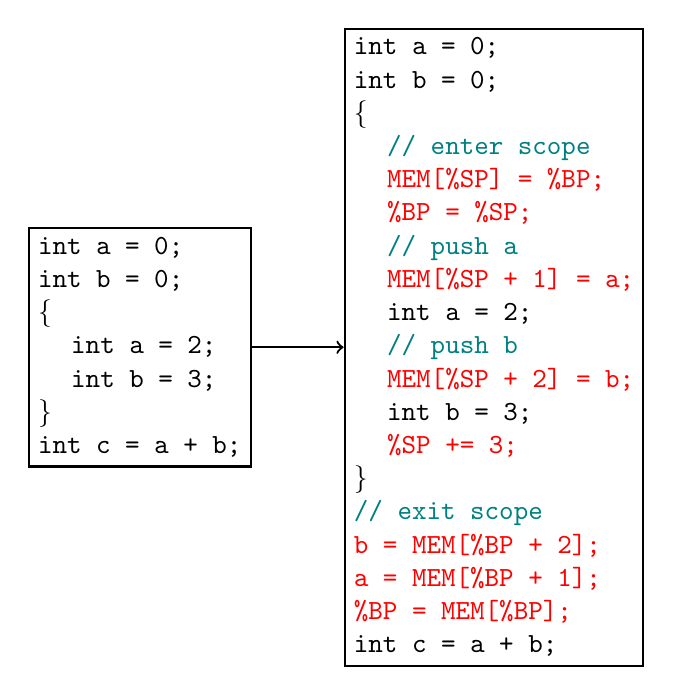
\begin{tikzpicture}[node distance={45mm}, thick, main/.style = {draw}] 
        \node[main, align=left] (Orig) {
            \code{int a = 0;}\\
            \code{int b = 0;}\\
            \code{\{}\\
            \code{\hspace{12pt}int a = 2;}\\
            \code{\hspace{12pt}int b = 3;}\\
            \code{\}}\\
            \code{int c = a + b;}
        };
        \node[main, align=left] (Scoped) [right of=Orig] {
            \code{int a = 0;}\\
            \code{int b = 0;}\\
            \code{\{}\\
            \comment{\hspace{12pt}// enter scope }\\
            \red{\code{\hspace{12pt}MEM[\%SP] = \%BP;}}\\
            \red{\code{\hspace{12pt}\%BP = \%SP;}}\\
            \comment{\hspace{12pt}// push a }\\
            \red{\code{\hspace{12pt}MEM[\%SP + 1] = a;}}\\
            \code{\hspace{12pt}int a = 2;}\\
            \comment{\hspace{12pt}// push b }\\
            \red{\code{\hspace{12pt}MEM[\%SP + 2] = b;}}\\
            \code{\hspace{12pt}int b = 3;}\\
            \red{\code{\hspace{12pt}\%SP += 3;}}\\
            \code{\}}\\
            \comment{// exit scope }\\
            \red{\code{b = MEM[\%BP + 2];}}\\
            \red{\code{a = MEM[\%BP + 1];}}\\
            \red{\code{\%BP = MEM[\%BP];}}\\
            \code{int c = a + b;}
        };
        \draw[->] (Orig) -- (Scoped);
    \end{tikzpicture} 
    \caption{A scope handling example for \CoBBl, where \code{MEM} represents the write-once memory used for stack simulation. Note that this transformation takes place only if \code{a} and \code{b} are selected by \CoBBl's register spilling.}
    \label{fig:continuation-passing}
\end{figure}

\subsection{Lowering segments into constraints} \label{sec:frontend_lowering}
For all non-memory instructions, \CoBBl~reuses the CirC compiler to lower them down to CirC IR. Memory operations in \CoBBl~are divided into two categories: those on the scope stack introduced by register spilling, and those on the virtual memory composed of allocated arrays. Virtual memory operations are expressed as in Buffet \cite{wahby14buffet} in a 4-tuple ($\addr$, $\val$, $\ls$, $\ts$), marking the address, value, whether the operation is a store or load, and the timestamp of the operation. Scope operations are only expressed as ($\addr$, $\val$), as the write-once memory representation ensures that every access to the same address will always yield the same value, regardless of the type of the operation, or when the operation takes place. 

%\section{Verifying the Constraints Efficiently}
The backend structure of \CoBBl~resembles that of vRAM, and can be divided into four components: correct execution of blocks, consistency of program states, permutation of the program states, and memory coherence. We present the full backend pipeline in figure \ref{fig:backend-overview}.

\begin{figure*}[htbp]
  \centering
  \hspace*{-1cm}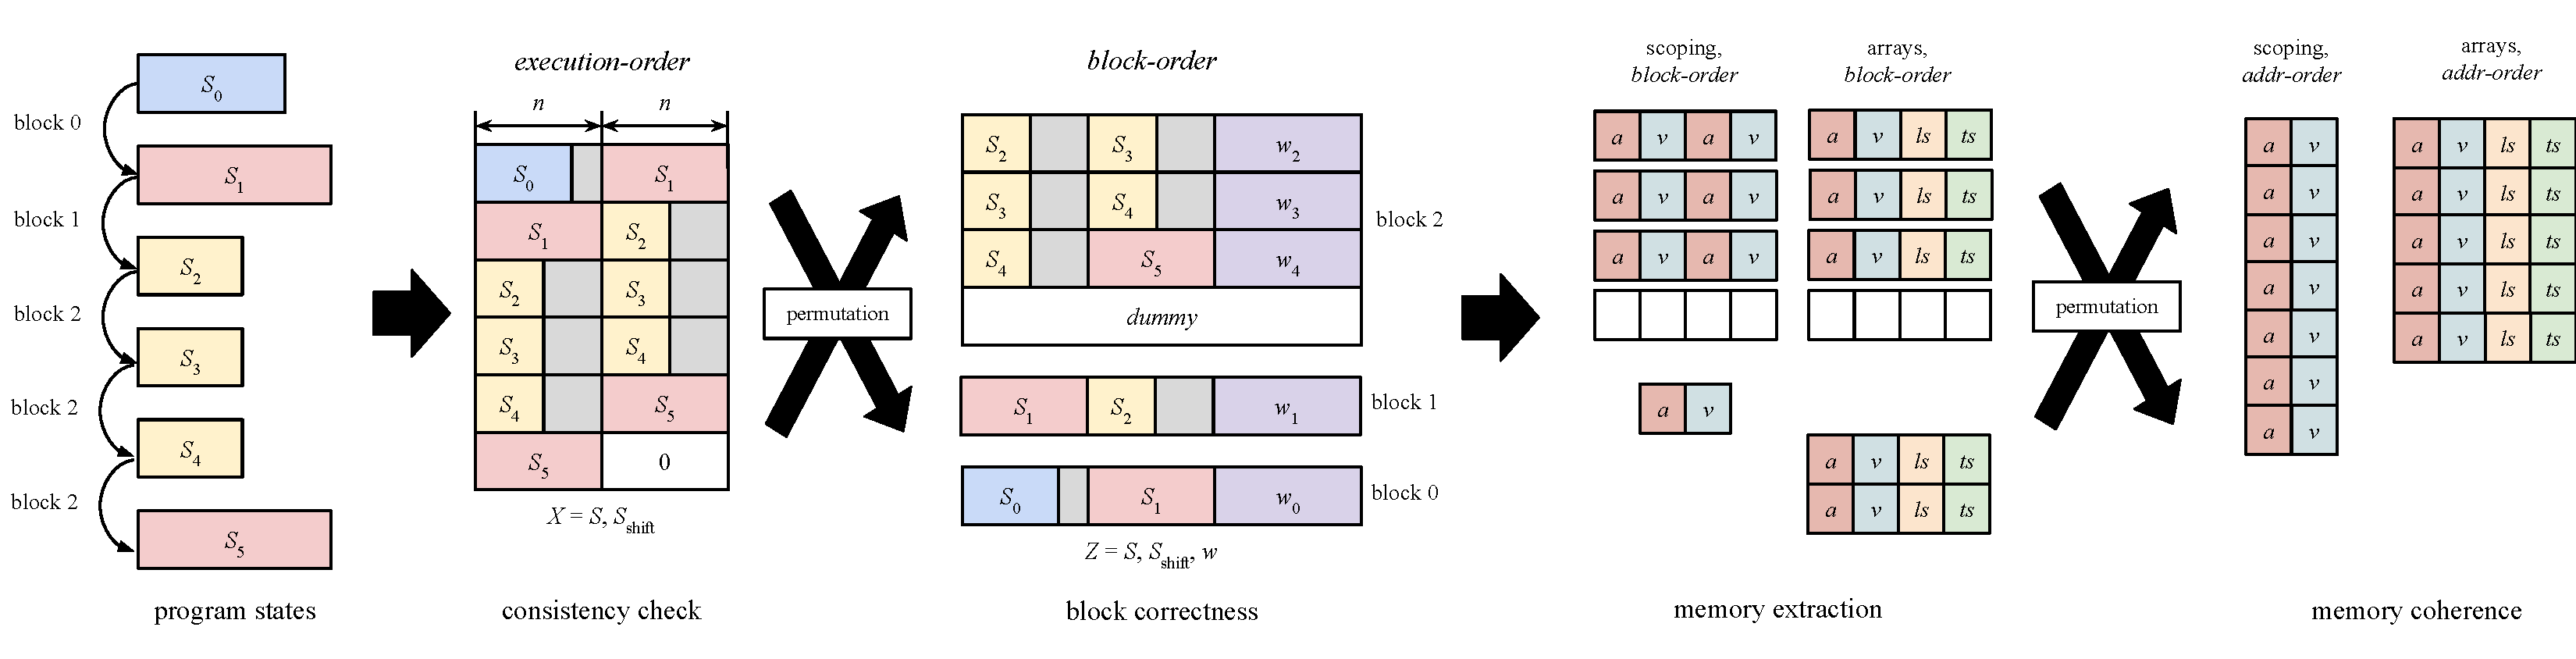
\includegraphics[width=\textwidth]{backend_overview.pdf}  
  \caption{Overview of the \CoBBl~backend.}
  \label{fig:backend-overview}
\end{figure*}

\subsection{Execution trace and witnesses}
For any execution of the \emph{preprocessed program}, \CoBBl~expresses the execution trace as a sequence of program states $[S_0\dots S_T]$, where $S_0$ is the program input and each subsequent state $S_{i+1}$ is produced by applying a block $I_i$ on the previous program state $S_i$. However, unlike vRAM, where each instruction sets a single output register, an execution of a block involves arbitrary side effects on all variables and an additional set of intermediate computations. As a result, to verify a block execution $I_i$, $\P$ computes $Z_i = (S_i, S_{i+1}, w_i)$ as witnesses for the proof, where $S_i$ is the prior program state and the input, $S_{i+1}$ is the next program state and the output, and $w_i$ contains all intermediate computations.

\subsection{Correct execution of blocks} \label{sec:block_correctness}
Verification of each individual block execution $I_i$, when singled out, is the exact same process as verifying a full program: a proof with constraints representing a block and witness represented as $Z_i = (S_i, S_{i+1}, w_i)$. Verification of multiple block executions in a data-paralleled proof, however, involves a few changes. The first is that, just like in vRAM, all executions of the same block need to be grouped together. This introduces a permutation described in section \ref{sec:perm}. Furthermore, number of executions of each block should be a power of 2 (or 0). These two properties allow the binary representation of the ordering to implicitly express the executed block. As an example, assume that the frontend emits 4 blocks: A, B, C, and D. For a particular computation, A is executed 8 times, B is executed 4 times, and C and D 2 times respectively. After sorting by block type, block correctness check verifies 16 executions in parallel, labeled as 0 to 15. To determine which block is applied to each program state, one refers to the binary of the label: if the first bit of the label is 0, then block A is in use; if the first two bits are 10, then B is in use, etc. Such implicit references avoid constraint description within each block execution.

Of course, the number of executions of most blocks are not a power of two. In this case $\P$ pads the proof with dummy executions where every witness is set to 0. This leads to a problem: constraints of every block need to be satisfiable by all-zero witnesses. Fortunately, this requirement is already satisfied by existing SNARK constraints, reasoned below:
\begin{itemize}
    \item If a constraint does not contain additions that involve constant values (i.e., it either performs arithmetic operations between witnesses, or multiplies a witness by a constant), then it can be satisfied by setting all witnesses to 0.
    \item To express additions with constant values, SNARK systems typically include a witness assigned to the constant 1 and perform addition using that witness. Since that witness is also set to 0 in a dummy execution, constraints with constant additions are also satisfiable by all-zero witnesses.
\end{itemize}

Finally, to ensure that $\P$ correctly sorts executions by block type, each block is assigned a label and each program state $S_i$ includes an additional register $\bn_i$ indicating the next block to be executed. Each block begins by checking that the value of $\bn_i$ matches with its label, and ends by setting $\bn_{i+1}$ to the label of the next block. If $\P$ incorrectly sorts or pads the executions, the check on $\bn_i$ fails, leading to a rejected proof.

\subsection{Consistency between program states} \label{sec:consistency}
The consistency check involves verifying that consecutive entries $Z_i = (S_i, s_{i+1}, w_i), Z_{i+1} = (S_{i+1}, s_{i+2}, w_{i+1})$ are consistent with each other, i.e. they share the same $S_{i+1}$. We note that $w_i$ plays no role in the consistency check, and does not need to be included. We pad each $S_i$ to width $n = \max_i|S_i|$. Let $X_i = (S_i, S_{i+1})$ so $|X_i| = 2n$, the goal of consistency check is to then show that
$$\forall k\in [0, n), X_i[n + k] = X_{i+1}[k]$$

Naively, the consistency proof seems easily parallelizable: each constraint of the consistency proof only uses variables from two consecutive entries $X_i$ and $X_{i+1}$. One can thus define the witnesses as $Y_i = (X_i, X_{i+1}) = (S_i, S_{i+1}, S_{i+1}, S_{i+2})$ and perform the following check in parallel across all $Y_i$:
$$\forall k\in [0, n), Y_i[n + k] = Y_i[2n + k]$$

However, such an approach only defers the problem from $X$ to $Y$. By expressing $Y_i = (X_i, X_{i+1})$, we now have to ask: how to prove that $Y_i$ and $Y_{i+1}$ share the same $X_{i+1}$?

Instead, \CoBBl~proves program state consistency through a \emph{proof of shift}. \CoBBl~represents each $X_i$ as a row in a $2n \times T$ matrix $X$. As shown in figure \ref{fig:backend-overview}, the matrix $X$ can be easily divided into two halfs: the left half is a matrix $S = S_0, \dots S_T$ and the right half is its shifted version $S_{\text{shift}} = S_1, \dots, S_T, 0$ differed by exactly one row ($n$ entries). \CoBBl~then generates the proof in the following manner:
\begin{enumerate}
    \item $\P$ provides $S$ and $S_{\text{shift}}$, and forms $X = S | S_{\text{shift}}$.
    \item $\P$ uses rows of $X$ as witnesses to produce a data-paralleled proof on program state consistency.
    \item $\P$ proves that $S_{\text{shift}}$ is $S$ shifted by $n$ entries.
\end{enumerate}

To prove that $S_{\text{shift}}$ is a shift of $S$, $\P$ interpolates both matrices as univariate polynomials $\tilde{S}, \tilde{S}_{\text{shift}}$ and evaluates them on a random point $r$. Let $\langle a, b \rangle$ denote vector dot product and
$$R = (1, r, r^2, r^3, \dots, r^n)$$
then
$$\tilde{S}(r) = \langle R, S_0 \rangle + r^n\cdot \langle R, S_1 \rangle + \dots + r^{(T-1)\cdot n} \langle R, S_T \rangle$$
$$\tilde{S}_{\text{shift}}(r) = \langle R, S_1 \rangle + r^n\cdot \langle R, S_2 \rangle + \dots + r^{(T-2)\cdot n} \langle R, S_T \rangle$$
So
$$\tilde{S}(r) = \langle R, S_0 \rangle + r^n \cdot \tilde{S}_{\text{shift}}(r)$$

Since $S_0$ is the program input already known by $\V$, $\V$ can manually compute $\langle R, S_0 \rangle$ and $r^n$. $\P$ provides $\tilde{S}(r)$ and $\tilde{S}_{\text{shift}}(r)$ through polynomial commitment, and $\V$ checks that $\tilde{S}(r) = \langle R, S_0 \rangle + r^n \cdot \tilde{S}_{\text{shift}}(r)$.

\bigskip
\noindent\textbf{Program input and output}. To conclude the consistency check, $\V$ needs to additionally check that the program input and output are correctly included in $S$. This is done by opening all relevant entries in $S_0$ and $S_T$ and verify their content.

\subsection{Permutation of program states} \label{sec:perm}
Since block execution check requires the program states to be sorted by block type, while consistency check requires the program states to be sorted by the order of execution, the next step is to verify that the two transcripts are indeed permutations of each other. Since the intermediate computations $w_i$ are only used in the block correctness proof, $w_i$ does not need to be part of the permutation. The permutation check is then reduced to the following problem: given two list of $(S_i, S_{i+1})$, how to prove that they are permutations of each other?

\CoBBl~reuses the idea of Reed-Solomon fingerprinting \cite{lipton90efficient}. Given two lists $a = (a_0, a_1, \dots, a_T), b = (b_0, b_1, \dots, b_T)$, to prove that they are permutations of each other, $\P$ constructs polynomials $A(i) = \prod_i(x - a_i)$ and $B(i) = \prod_i(x - b_i)$. $\V$ then evaluates them on a random point $\tau$. If $a$ and $b$ are permutations, then $A$ and $B$ are the same polynomial, so $A(\tau) = B(\tau)$. If $a$ and $b$ are not permutations, then $A$ and $B$ are different polynomials, and the likelihood of them agreeing on a random point is negligibly low.

To expand this idea onto $S$, where each entry of the lists are program states instead of a single number, $\CoBBl$ first performs \emph{the same random linear combination} on each program state to obtain $\text{RLC}(S_i) = \sum_k r^k s_{i, k}$. The remaining steps are now equivalent to that of a regular fingerprinting: construct two polynomials from $\text{RLC}_{\text{block}}$ and $\text{RLC}_{\text{exec}}$, and verify the equivalence of their evaluation on a random point $\tau$.

\subsection{Memory Coherence}
\CoBBl's memory coherence check closely resembles those of Buffet: for every load on an address, the value obtained should be the same as the last value loaded from or stored to that address. To verify this, \CoBBl~invokes a three-step process: extraction, permutation, and pairwise memory coherence check.

\paragraph{Extraction} The first step is to extract all memory accesses from the execution. As described in section \ref{sec:frontend_lowering}, memory accesses in \CoBBl~are separated into two categories: those on the scope stack and those on arrays. Operations on the scope stack are expressed using the pair $(\addr, \val)$, while operations on arrays are described by $(\addr, \val, \ls, \ts)$. Fortunately, since constraints for each block is fixed at compile time, for each block execution, \CoBBl~knows exactly where each memory variable is located. All that remains is for the frontend to append additional constraints to the end of each block, extracting out all scoping and array operations into a list of 2-tuples and a list of 4-tuples.

\paragraph{Permutation} The goal of the permutation is to allow $\P$ to sort all memory accesses by their addresses, on which the final coherence check will be performed. We note that this step is inherently identical to the process described in section \ref{sec:perm}. At the end of the permutation proof, $\P$ convinces $\V$ that a list of scoping accesses $L_{\text{scope}}$ and a list of array accesses $L_{\text{array}}$ contain all memory operations executed during the computation.

\paragraph{Pairwise coherence check} With lists of memory accesses purportedly sorted by their addresses, the final check is consisted of two steps. $\V$ first checks that the lists are sorted correctly: for $L_{\text{scope}}$, addresses should be increasing and differ by at most 1; for $L_{\text{array}}$, addresses should be increasing, and accesses on the same address is tie-breaked by the timestamp. The second check is on coherence: for $L_{\text{scope}}$, consecutive accesses on the same address should always result in the same value, and for consecutive accesses on the same address in $L_{\text{scope}}$, if the second access is a load, then the value of the second access should match that of the first. If both checks pass, then $\V$ is convinced of memory coherence.

%As a result, the proof includes the following witnesses from $\P$:
%\begin{itemize}
%    \item A list of program states $[S_0\dots S_T]$, sorted in the order of execution.
%    \item A list of consecutive program state pair $(S_i, S_{i+1})$, sorted by the type of block executed between the pair.
%    \item A list intermediate computations $z_i$ corresponding to the $(S_i, S_{i+1})$ pair.
%\end{itemize}


\section{Evaluation}

Our experiment with \CoBBl~aims to answer the following questions:
\begin{enumerate}
  \item How does \CoBBl~perform compare to state-of-the-art direct-translators on (a) compiler time, (b) prover time (c) verifier time, and (d) proof size? \label{q:performance-dt}
  \item How does \CoBBl~perform compare to state-of-the-art virtual machines on the same metrics as in question \ref{q:performance-dt}? \label{q:performance-vm}
  \item To what extent do improvements introduced through \CoBBl's block-based abstractions outweight the overheads? \label{q:tradeoff}
  \item How effective are \CoBBl's static optimizations in improving proof runtime and size? \label{q:optimization}
\end{enumerate}

We choose CirC~\cite{ozdemir20circ} as the baseline for state-of-the-art direct translator, and Jolt~\cite{arun23jolt} as the baseline for virtual machine. \red{[XXX: Need justification?]} We conduct the experiments on implementations of \CoBBl, CirC and Jolt across several benchmarks.

\subsection{Implementation}
\red{[XXX: Will there be a separate implementation section? Some details might be interesting to go through]} We base the frontend compiler of \CoBBl~on top of existing infrastructure of CirC, our direct translator baseline, as CirC contains most underlying functionalities required by \CoBBl~(in particular, conversion of high-level languages to constraints). On top of CirC, we implement \CoBBl's frontend through 7000 lines of Rust code: dividing a program in to segments, performing all optimizations on each segment, and repackaging each segment as individual programs recognizable by CirC's direct translator. We apply minimal modification to CirC's internal codebase to ensure fairness of comparison.

The backend proof system for \CoBBl~is a custom variant of Spartan~\cite{setty19spartan}, the same proof system used by our two baselines. We modify Spartan through 7000 lines of Rust code to support parallel execution of all program segments, but leave most internal logic untouched.

\subsection{Baselines and Benchmarks}
\paragraph{CirC} We modify CirC to support branching statements to align with our benchmarks, but using exclusively existing functionalities. Apart from updates to the parser and input format, everything else stays the same as the original codebase~\cite{circ_codebase}.

\paragraph{Jolt} Our Jolt evaluation uses the released codebase~\cite{jolt_codebase}.

\paragraph{\CoBBl~without optimization} To answer question \ref{q:optimization}, we disable all non-essential \CoBBl~optimizations (most importantly, block merge and register spilling) and conduct tests across all benchmarks.

\paragraph{Benchmarks} Figure \ref{fig:benchmark_overview} lists our benchmarks. We implement each benchmark in two programming languages: the Zokrates version is used by \CoBBl~and CirC, while Jolt uses the Rust version, compiled using release mode (\code{--release}). As Zokrates closely resembles Rust, the two versions of each benchmark are identical up to grammatical difference. Since CirC generally performs far worse than Jolt, we choose a different set of parameters when comparing \CoBBl~against CirC and Jolt. All benchmarks except for Poseidon are computed exclusively using 32-bit registers -- the native instruction set for Jolt -- to ensure its maximum efficiency. We explore the special scenario introduced by Poseidon later in the section.

\paragraph{Special Benchmark} To answer question \ref{q:tradeoff}, we conduct a separate test on the Find Min benchmark, recording performance of CirC and \CoBBl~for array length ranging from 200 to 1600.

\begin{table}[t]
  \begin{tabular}{l l l}
    \centering
    \textbf{Benchmarks} & \textbf{Parameters} & \textbf{Type} \\
    \hline \\
    \makecell[l]{Min value in an array \\ (Find Min)} & \makecell[l]{\emph{v. CirC}: len = 1200 \\ \emph{v. Jolt}: len = 1200} & 32-bit \\
    \vspace{2\baselineskip}\\
    \makecell[l]{Matrix Multiplication \\ (Mat Mult)} & \makecell[l]{\emph{v. CirC}: size = 8x8 \\ \emph{v. Jolt}: size = 16x16} & 32-bit \\
    \vspace{2\baselineskip}\\
    \makecell[l]{KMP pattern match \\ (Pat Match)} & \makecell[l]{\emph{v. CirC}: pat / txt = 48 / 480 \\ \emph{v. Jolt}: pat / txt = 48 / 480} & 32-bit \\
    \vspace{2\baselineskip}\\
    \makecell[l]{Largest common subsequence \\ (LCS)} & \makecell[l]{\emph{v. CirC}: len = 5 \\ \emph{v. Jolt}: len = 30} & 32-bit \\
    \vspace{2\baselineskip}\\
    \makecell[l]{RLE encode + decode \\ (RLE)} & \makecell[l]{\emph{v. CirC}: len = 20 \\ \emph{v. Jolt}: len = 60} & 32-bit \\
    \vspace{2\baselineskip}\\
    \makecell[l]{Sha-256 Hashing \\ (Sha256)} & \makecell[l]{\emph{v. CirC}: len = 1 \\ \emph{v. Jolt}: len = 6} & 32-bit \\
    \vspace{2\baselineskip}\\
    \makecell[l]{Poseidon Hashing \\ (Poseidon)} & \makecell[l]{\emph{v. CirC}: len = 3 \\ \emph{v. Jolt}: len = 6} & field \\
  \end{tabular}
  \caption{Overview of benchmarks.}
  \label{fig:benchmark_overview}
\end{table}

\subsection{Setup}
Our testbed is a MacBook pro running on a 10-core M1 Max chip and 64 GB of memory. For each system and benchmark, we execute the computation 5 times, recording compiler, prover, verifier time, and proof size and averaging the results. 

\subsection{Method and Results}
\subsubsection{Comparing Runtime of \CoBBl~with CirC}
We present the performance comparison in figure \ref{fig:performance_dt}. \red{[XXX: Fix overlap on graph]} For each benchmark, we measure the compiler, prover, and verifier time of \CoBBl~as speedups from CirC. Since runtime of \CoBBl~scales with program input but runtime of CirC stays the same, we derive three scenarios regarding to the workload of \CoBBl:
\begin{itemize}
  \item \textbf{CoBBl For} executes the exact same program as CirC, where the size of the array and number of iterations of each loop is statically bounded.
  \item \textbf{CoBBl 75} sets the array size to be 75\% of the statically inferred upper bound. Subsequently, all loops are executed only 75\% of the statically inferred number of iterations. \red{[XXX: Need to talk about the exception of Mat Mult.]}
  \item \textbf{CoBBl 50} is similar to CoBBl 75, but with only 50\% array size.
\end{itemize}

To enhance CirC's performance, we allow polynomial commitment in both \CoBBl~and CirC to run in multicore. We note that since polynomial commitment takes up a higher percentage of CirC's runtime than \CoBBl, such a setup is more beneficial towards CirC.

\begin{figure*}[t]
  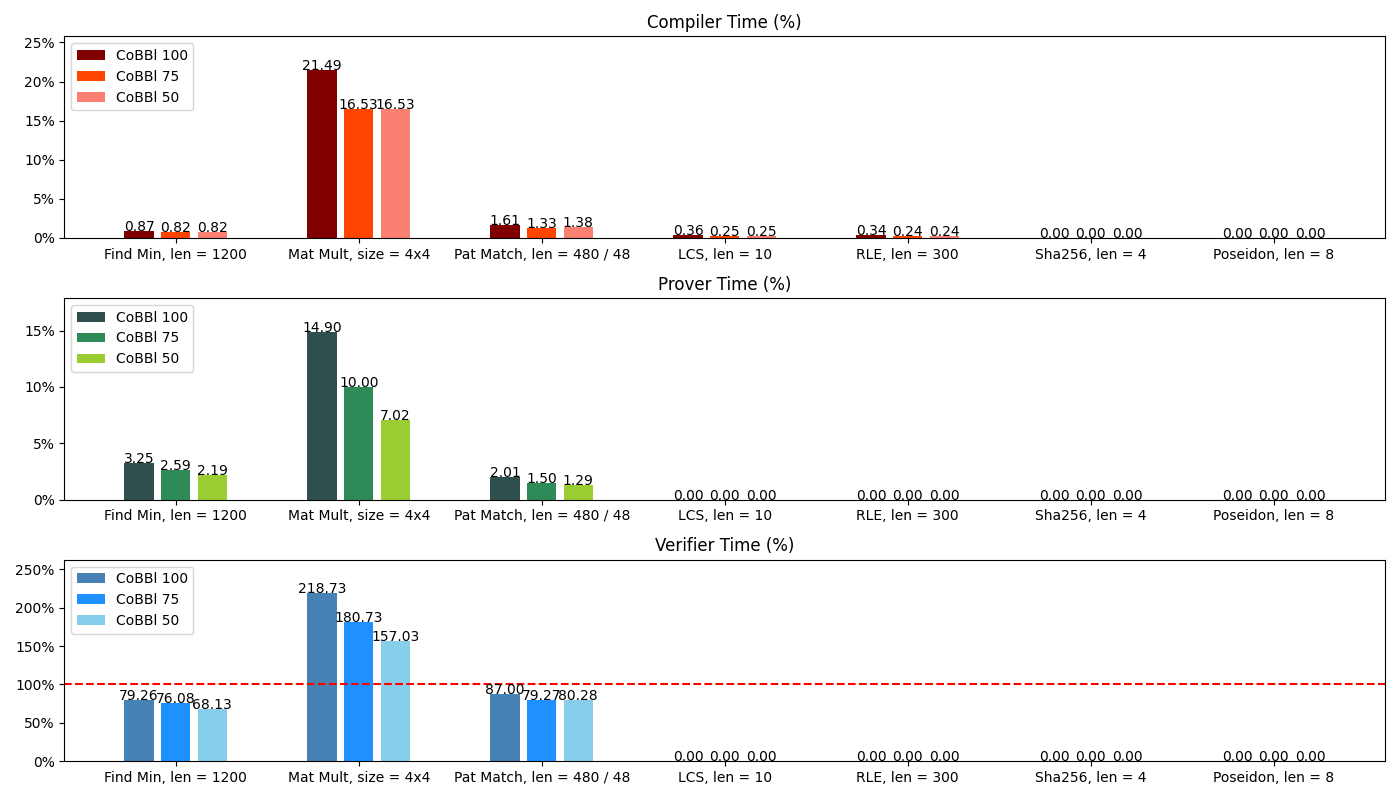
\includegraphics[width=\textwidth]{graph/fig_eval_circ.png}
  \caption{Runtime comparison between \CoBBl~and CirC.}
  \label{fig:performance_dt}
\end{figure*}

%\section{Conclusion}
This paper introduces \CoBBl, a SNARK system that combines program-specific optimizations with execution-path-specific constraints. We acknowledge that \CoBBl~is an enormous system developed by a single grad student, and thus, demands a long development cycle. While a prototype of \CoBBl~is close to completion, there are still endless opportunities for future optimizations on both the compiler and on creating a more efficient backend protocol. Preliminary testings have shown that the performance of \CoBBl~is on par with state-of-the-art SNARK compilers. We hope that future work on \CoBBl~can further improve the efficiency of the system, bringing it closer to industrial standard.

\bibliography{references}
\bibliographystyle{alpha}

\end{document}
